%%
%% Copyright 2007, 2008, 2009 Elsevier Ltd
%%
%% This file is part of the 'Elsarticle Bundle'.
%% ---------------------------------------------
%%
%% It may be distributed under the conditions of the LaTeX Project Public
%% License, either version 1.2 of this license or (at your option) any
%% later version.  The latest version of this license is in
%%    http://www.latex-project.org/lppl.txt
%% and version 1.2 or later is part of all distributions of LaTeX
%% version 1999/12/01 or later.
%%
%% This template has been modified by Philip Blakely for
%% local distribution to students on the MPhil for Scientific
%% Computing course run at the University of Cambridge.
%%

%% Template article for Elsevier's document class `elsarticle'
%% with numbered style bibliographic references
%% SP 2008/03/01
%%
%%
%%
%% $Id: elsarticle-template-num.tex 4 2009-10-24 08:22:58Z rishi $
%%
%%
\documentclass[final,3p,times,twocolumn]{elsarticle}

%% Use the option review to obtain double line spacing
%% \documentclass[preprint,review,12pt]{elsarticle}

%% Use the options 1p,twocolumn; 3p; 3p,twocolumn; 5p; or 5p,twocolumn
%% for a journal layout:
%% \documentclass[final,1p,times]{elsarticle}
%% \documentclass[final,1p,times,twocolumn]{elsarticle}
%% \documentclass[final,3p,times]{elsarticle}
%% \documentclass[final,3p,times,twocolumn]{elsarticle}
%% \documentclass[final,5p,times]{elsarticle}
%% \documentclass[final,5p,times,twocolumn]{elsarticle}

%% if you use PostScript figures in your article
%% use the graphics package for simple commands
%% \usepackage{graphics}
%% or use the graphicx package for more complicated commands
\usepackage{graphicx}
%% or use the epsfig package if you prefer to use the old commands
%% \usepackage{epsfig}

%% The amssymb package provides various useful mathematical symbols
\usepackage{amssymb}
%% The amsthm package provides extended theorem environments
%% \usepackage{amsthm}

%% The lineno packages adds line numbers. Start line numbering with
%% \begin{linenumbers}, end it with \end{linenumbers}. Or switch it on
%% for the whole article with \linenumbers after \end{frontmatter}.
%% \usepackage{lineno}

%% natbib.sty is loaded by default. However, natbib options can be
%% provided with \biboptions{...} command. Following options are
%% valid:

%%   round  -  round parentheses are used (default)
%%   square -  square brackets are used   [option]
%%   curly  -  curly braces are used      {option}
%%   angle  -  angle brackets are used    <option>
%%   semicolon  -  multiple citations separated by semi-colon
%%   colon  - same as semicolon, an earlier confusion
%%   comma  -  separated by comma
%%   numbers-  selects numerical citations
%%   super  -  numerical citations as superscripts
%%   sort   -  sorts multiple citations according to order in ref. list
%%   sort&compress   -  like sort, but also compresses numerical citations
%%   compress - compresses without sorting
%%
%% \biboptions{comma,round}

% \biboptions{}

\usepackage{amsmath}
\numberwithin{equation}{section}

\journal{MPhil in Scientific Computing}

\begin{document}

\begin{frontmatter}

%% Title, authors and addresses

%% use the tnoteref command within \title for footnotes;
%% use the tnotetext command for the associated footnote;
%% use the fnref command within \author or \address for footnotes;
%% use the fntext command for the associated footnote;
%% use the corref command within \author for corresponding author footnotes;
%% use the cortext command for the associated footnote;
%% use the ead command for the email address,
%% and the form \ead[url] for the home page:
%%
%% \title{Title\tnoteref{label1}}
%% \tnotetext[label1]{}
%% \author{Name\corref{cor1}\fnref{label2}}
%% \ead{email address}
%% \ead[url]{home page}
%% \fntext[label2]{}
%% \cortext[cor1]{}
%% \address{Address\fnref{label3}}
%% \fntext[label3]{}

\title{A Full Configuration Interaction Quantum Monte-Carlo Algorithm applied to the Uniform Electron Gas}

%% use optional labels to link authors explicitly to addresses:
%% \author[label1,label2]{<author name>}
%% \address[label1]{<address>}
%% \address[label2]{<address>}

\author{Alexander Card}

\address{Department of Chemistry, Lensfield Road, Cambridge CB2 1EW}

\begin{abstract}
This report describes an application of the FCIQMC algorithm specifically applied to the UEG, the more general motivation of the FCIQMC method, its theoretical foundations stemming from FCI, and finer algorithmic details. Nuances of the particular algorithm written entirely from scratch in C++ and specifically for this report will be covered. A projection of the possible scope of the code, as well as desired computational improvements will be given. Results obtained for the UEG system using the code written for this report will be compared to literature, and from this will follow a discussion on their validity. 14 Electrons are used throughout, and densities of $r_s$ 0.5 and 1.0 are studied at a variety of plane-wave basis energy cutoffs. The most interesting points of the algorithm's nature are discussed with respect to some possible input parameters in order to give a sense of the most efficient way to implement this code, and advantages of FCIQMC over deterministic methods for obtaining ground-state eigenvalues is given.
\end{abstract}

\end{frontmatter}

%%
%% Start line numbering here if you want
%%
% \linenumbers

%% main text
\section{Introduction and Background Theory}
FCIQMC is a stochastic method derived directly from the determinisitc FCI method for finding the lowest eigenvalue of the Hamiltonian matrix, for a given system. It is designed in such a way as to converge upon the true FCI wavefunction and eigenvalue, given a exhaustive sampling of the full Slater-determinant space, $\{D_I\}$, over a long time, ($\tau \rightarrow \infty$) , which solve the imaginary-time schrodinger equation
\begin{equation}
\frac{\partial \Psi }{\partial \tau} = -\hat H \Psi
\end{equation}
This innocuous equation can be trivially solved and then shown to express the imaginary-time-dependent wavefunction, which uses a reference wavefunction (a Slater determinant of with the same symmetry as the ground-state) to propogate out the exact lowest energy, $E_{GS}$ of the system :
\begin{equation}
\Psi(\tau) = e^{-\tau(\hat H - E_{GS})}|\Psi_{\tau = 0} \rangle 
\end{equation}
where $e^{-\tau(\hat H)}$ is effectively the propagation operator which, in the limit of infinite time, will give the exact ground state. The ground state, or FCI, wavefunction therefore must be dealt with in terms of Slater-determinants, whose value is simply the sum of all energetically contributing Slater determinants:
\begin{equation}
\Psi_{FCI} = \sum_{I} c_I (\tau) | D_I \rangle
\end{equation}
FCIQMC uses stochastic methods to numerically integrate equation 1.1, which, in the language of Slater determinants corresponds to the following master equation:
\begin{equation}
-\frac{\partial c_I}{\partial \tau} = (H_{II} - E_{ref}\delta_{IJ} - S) + \sum_{I \neq J} c_I H_{IJ}
\end{equation}

S is termed the Shift, and simultaneously controlles the population dynamics, and gives one measure of the correlation energy of the system. For simplicity, and future reference, the matrix \textbf{K} is defined as having elements $K_{IJ} = \langle D_I | \hat K | D_J \rangle = \langle D_I | \hat H | D_J \rangle - E_{ref}\delta_{IJ} $.  
The reference determinant, whose energy is $E_{ref}$, is in this report always chosen as the Hartree-Fock determinant, which is defined as the determinant representing the electronic filling of the lowest possible energy states.\\

It is now clear that the coefficients $\{c_I\}$ , and crucially their signs, determine the true wavefunction. FCIQMC thus simulates this set of coefficients by associating each one with a population of imaginary particles, which will be henceforth referred to as Walkers. The number (and sign) of these walkers is associated with a particular determinant in the set which make up the FCI wavefunction, and the FCIQMC algorithm grows a population of these walkers and allows them to evolve through the full space of possible Slater determinants, until a suffucient population (corresponding to a sufficient number of terms equation 1.3) is reached. The number of walkers on a certain determinant $D_J$ is proportional to its theoretical coefficient $c_J, c_J \propto Nw_{D_J} $,  (theoretical in the sense that the FCIQMC algorithm is only aware of walkers, and is completely ignorant of the coefficients it simulates). Thus, a population dynamics algorithm controlling the evolution of these walkers in Slater-deteminant space is the heart of the FCIQMC algorithm.


It is important to note that, although a numerical method, the complete and deterministic nature of FCI means that it is able to give fundamentally exact results (for a given, finite, basis set). The caveat is of course that the combinatorics involved with calculating all possible excitations of a system and the corresponding Hamiltonian matrix render is legitimately impossible to be used for a large system.



\subsection{SUBSECTION}
The instantaneous projector energy estimator is given by

\begin{equation}
E_{proj} = \frac{1}{N_0} \sum_I \  \langle D_0 | H | D_I \rangle N_I
\end{equation}

and the mean projector energy estimator as a function of imaginary time is given by the following, where it is important to note that the averages of the reference and Ith determinant's populations must be averaged separately:


\begin{equation}
\langle E_{proj}(\tau) \rangle = \frac{1}{\langle N_0(\tau) \rangle}  \sum_I \  \langle D_0 | H | D_I \rangle \langle N_I(\tau) \rangle
\end{equation}




\section{Mathematical formulae}
\label{sect:Formulae}
Complex formulae are easy to produce within \LaTeX{}. For example, we
can use inline equations to define $f(x) = a_3x^3 + a_2x^2 + a_1x +
a_0$, and then provide more complex equations such as
\begin{equation}
\int_0^3 f(x) \mathrm{d}x = \left[\frac{a_3}{4}x^4 + \frac{a_2}{3}x^3
  + \frac{a_1}{2}x^2 + a_0x\right]_0^3
\label{eqn:Taylor}
\end{equation}
If we have some derivation that should belong elsewhere, we can put it
in an appendix such as \ref{app:quad}. We can also refer to equations
from the main text such as the Taylor expansion \ref{eqn:Taylor}.
\section{Pictures}
\label{sect:Pictures}
In this section we demonstrate the inclusion of figures. For example,
Figure~\ref{fig:ENO1} demonstrates ENO as used to solve a linear advection
of a top-hat function.
\begin{figure}
\centering
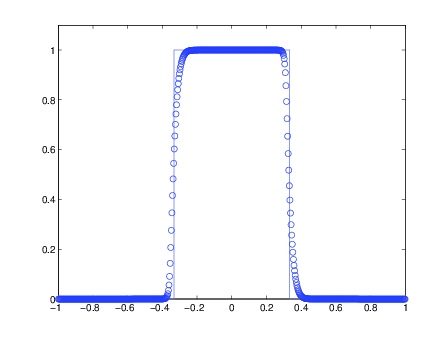
\includegraphics[width=3in]{ENOTest3b.png}
\caption{Demonstration of ENO as used to solver linear-advection of a
  top-hat function.}
\label{fig:ENO1}
\end{figure}
\section{Conclusions}
\label{sect:Concl}
In which we conclude that LaTeX (or \LaTeX) is very useful for
generating scientific papers as demonstrated above.

\section*{Acknowledgements}
Here I acknowledge the assistance of my supervisor, my industrial sponsor,
and the effects of caffeine on my ability to produce this report on time.

%% The Appendices part is started with the command \appendix;
%% appendix sections are then done as normal sections
\appendix

\section{On the Derivation of the Quadratic Formula}
\label{app:quad}
The derivation of the quadratic formula is something that would not
fit well within a paper as it would interrupt the flow of the argument
therein. However, for those students who need a refresher on how the
quadratic formula is derived, we give full details here:\par
Assume that we have
\begin{equation}
p(x) = ax^2 + bx + c
\end{equation}
and so on. The actual algebra is left as an exercise for the reader.

%% References
%%
%% Following citation commands can be used in the body text:
%% Usage of \cite is as follows:
%%   \cite{key}         ==>>  [#]
%%   \cite[chap. 2]{key} ==>> [#, chap. 2]
%%

%% References with bibTeX database:

\bibliographystyle{elsarticle-num}
\bibliography{references.bib}

%% Authors are advised to submit their bibtex database files. They are
%% requested to list a bibtex style file in the manuscript if they do
%% not want to use elsarticle-num.bst.

%% References without bibTeX database:

% \begin{thebibliography}{00}

%% \bibitem must have the following form:
%%   \bibitem{key}...
%%

% \bibitem{}

% \end{thebibliography}


\end{document}


%%
%% End of file `elsarticle-template-num.tex'.